\documentclass[tikz,border=10pt]{standalone}
\begin{document}
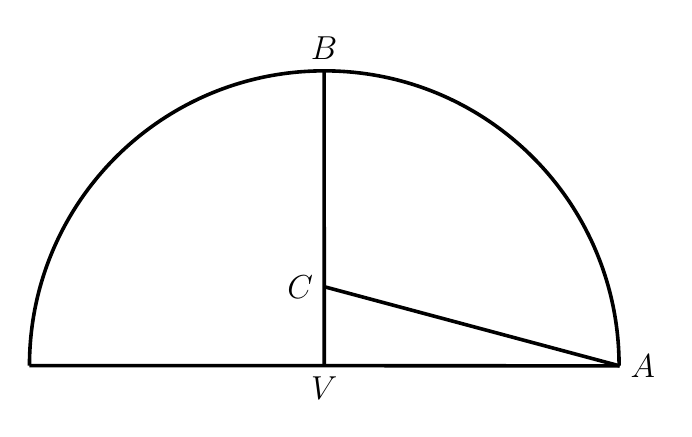
\begin{tikzpicture}[line join=round, line width=1.3pt]
\coordinate (A) at (3.428,-1.863);
\coordinate (B) at (-0.325,1.887);
\coordinate (C) at (-0.325,-0.857);
\coordinate (V) at (-0.323,-1.860);




\coordinate (L) at (-4.067,-1.860);


\draw (L) -- (V) -- (A);


\draw (V) ++(180.000:3.744) arc[start angle=180.000, end angle=0.000, radius=3.744];


\draw (B) -- (V);
\draw (A) -- (C);


\node[right, font=\fontsize{13}{15.6}\selectfont] at (A) {$A$};
\node[above, font=\fontsize{13}{15.6}\selectfont] at (B) {$B$};
\node[left, font=\fontsize{13}{15.6}\selectfont] at (C) {$C$};
\node[below, font=\fontsize{13}{15.6}\selectfont] at (V) {$V$};
\end{tikzpicture}
\end{document}